\documentclass[scheme=plain]{ctexart}
% Packages
\usepackage{xeCJK}
    \setCJKmainfont[AutoFakeBold,AutoFakeSlant]{KaiTi}
\usepackage{booktabs}
\usepackage{tabularx}
\usepackage[table]{xcolor}
\usepackage{geometry}
    \geometry{margin=1in}
\usepackage{multicol}
\usepackage{tcolorbox}
\usepackage{graphicx,subcaption,float}
    \graphicspath{{figures/}}
\usepackage{hyperref}
\usepackage{amsmath}
\usepackage{tcolorbox}
    \tcbuselibrary{theorems}
    \newtcbtheorem[number within=section]{analysis}{Analysis}%
        {colback=orange!5!white,colframe=orange!70!white,fonttitle=\bfseries}{A}
% Commands
\newcommand{\SUSTech}{
\includegraphics[height=2ex]{logo}}
% Information
\title{How Different Factors Influence Undergraduates on Playing Computer Games}
\author{}
\date{\today}
\begin{document}
\maketitle\tableofcontents\clearpage

\section{Purpose and Sampling}
In general, playing computer games is supposed to highly correlated with the undergraduates' study. In order to investigate how different factors influence undergraduates on playing computer games, we conducted a survey and focused on how long a \SUSTech\ student spent in playing computer games within one week under different preferences. Questionnaire was designed and 93 responses were received before data analysis.

Before implement our questionnaire, we first identified the target population, element, sampling unit, frame, sampling method of our sampling survey, which are listed below.
\begin{itemize}
    \item Population: the whole undergraduates of \SUSTech\
    \item Element: an individual student of \SUSTech\
    \item Sampling unit: an individual student of \SUSTech\
    \item Frame: a list of all undergraduates of \SUSTech\
    \item Sampling method: Stratified random sampling
    \item Stratas: split the whole undergraduates into 4 grades (freshman,sophomore,junior,senior), each grade is defined as a strata.
\end{itemize}

The questionnaire consists of 18 questions intended to go to detail of undergraduates playing computer games. For instance, what kinds of computer games does the interviewees like most, or would they make a plan about their playtime allocation. The complete questionnaire is listed below.

\begin{tcolorbox}
    \begin{multicols}{2}
        \begin{enumerate}
            \item 您的性别
            \item 您的年龄
            \item 您的年级
            \item 您所在院系或意向院系
            \item 您每周大概玩多长时间游戏(整数,以小时计)
            \item 您平时玩游戏的类型
            \item 您玩游戏的原因是
            \item 您是自己玩还是和朋友开黑
            \item 玩游戏前有对玩游戏这件事进行计划吗
            \item 玩游戏有固定的时间吗
            \item 您会熬夜打游戏吗(熬夜指晚上12:00以后)
            \item 在哪些情况下,您会熬夜打游戏
            \item 您一般几点睡
            \item 您熬夜是因为打游戏吗
            \item 您觉得自己打游戏影响到自己的学习生活了吗
            \item 您觉得自己打游戏有没有影响到他人的学习生活
            \item 您觉得别人打游戏有没有影响到您的学习生活
            \item 有因为自己或他人打游戏和周围的人发生过矛盾吗
        \end{enumerate}
    \end{multicols}
\end{tcolorbox}

Futhermore, the explanation of symbols can be seen in table~\ref{T:symbols-explanation}.
\begin{table}[H]
        \centering
        \begin{tabularx}{.8\textwidth}{cX}
                \toprule
                Symbol                                 & Explanation                                                      \\ \midrule
                \rowcolor[HTML]{EFEFEF} $X_{1}$        & Gender                                                           \\
                                        $X_{2}$        & Age                                                              \\
                \rowcolor[HTML]{EFEFEF} $X_{3}$        & Grade                                                            \\
                                        $X_{4}$        & Apartment or desired apartment                                   \\
                \rowcolor[HTML]{EFEFEF} $X_{5}$        & Hours spend on playing games per week                            \\
                                        $X_{6}^{(1)}$  & The game type usually play is MOBA                               \\
                \rowcolor[HTML]{EFEFEF} $X_{6}^{(2)}$  & The game type usually play is FPS                                \\
                                        $X_{6}^{(3)}$  & The game type usually play is RPG                                \\
                \rowcolor[HTML]{EFEFEF} $X_{6}^{(4)}$  & The game type usually play is card games                         \\
                                        $X_{6}^{(5)}$  & The game type usually play is webgames                           \\
                \rowcolor[HTML]{EFEFEF} $X_{6}^{(6)}$  & The game type usually play is console games                      \\
                                        $X_{6}^{(7)}$  & Usually play other games                                         \\
                \rowcolor[HTML]{EFEFEF} $X_{6}^{(8)}$  & Student who don't play games                                     \\
                                        $X_{7}^{(1)}$  & The reason of playing games is to release pressure               \\
                \rowcolor[HTML]{EFEFEF} $X_{7}^{(2)}$  & The reason of playing games is to kill time                      \\
                                        $X_{7}^{(3)}$  & The reason of playing games is having passion for games          \\
                \rowcolor[HTML]{EFEFEF} $X_{7}^{(4)}$  & The reason of playing games is to follow e-sport trend           \\
                                        $X_{7}^{(5)}$  & Driven by friends                                                \\
                \rowcolor[HTML]{EFEFEF} $X_{7}^{(6)}$  & Invited by friends                                               \\
                                        $X_{7}^{(7)}$  & Other reasons                                                    \\
                \rowcolor[HTML]{EFEFEF} $X_{7}^{(8)}$  & Student who don't play games                                     \\
                                        $X_{8}^{(1)}$  & Tend to play alone                                               \\
                \rowcolor[HTML]{EFEFEF} $X_{8}^{(2)}$  & Tend to play with friends                                        \\
                                        $X_{8}^{(3)}$  & Can play alone or play with friends                              \\
                \rowcolor[HTML]{EFEFEF} $X_{8}^{(4)}$  & Student who don't play games                                     \\
                                        $X_{9}$        & Whether have plan before play games                              \\
                \rowcolor[HTML]{EFEFEF} $X_{10}$       & Whether have settled playing time                                \\
                                        $X_{11}$       & Whether stay-up to play                                          \\
                \rowcolor[HTML]{EFEFEF} $X_{12}^{(1)}$ & Will stay-up to play when there is little learning task          \\
                                        $X_{12}^{(2)}$ & Will stay-up to play when want to achieve certain goals in games \\
                \rowcolor[HTML]{EFEFEF} $X_{12}^{(3)}$ & Will stay-up to play when made a promise with friends            \\
                                        $X_{12}^{(4)}$ & Others                                                           \\
                \rowcolor[HTML]{EFEFEF} $X_{12}^{(5)}$ & Don't stay-up to play games                                      \\
                                        $X_{13}$       & Time to sleep (Time interval between choices is 1 hour)          \\
                \rowcolor[HTML]{EFEFEF} $X_{14}^{(1)}$ & Due to playing games                                             \\
                                        $X_{14}^{(2)}$ & Don't due to playing games                                       \\
                \rowcolor[HTML]{EFEFEF} $X_{14}^{(3)}$ & Sometimes due to playing games                                   \\
                                        $X_{14}^{(4)}$ & Don't stay-up                                                    \\
                \rowcolor[HTML]{EFEFEF} $X_{15}$       & The influence to the player brought by playing games             \\
                                        $X_{16}$       & The influence to others brought by playing games                 \\
                \rowcolor[HTML]{EFEFEF} $X_{17}$       & The influence brought by others                                  \\
                                        $X_{18}$       & Whether had conflicts with others caused by games                \\ \bottomrule
        \end{tabularx}
        \caption{Symbols Explanation}\label{T:symbols-explanation}
\end{table}



\section{Data Pre-Analysis}
\subsection{Data Prior Analysis}
Our data pre-processing goal is to obtain a prior sample variance of each grade. After that we are able to obtain the sample size n such that the estimated avarage playtime is within an error bound $B$.

\begin{table}[htbp]
    \centering
    \begin{tabular}{|l|l|l|l|l|}
        \hline
        Play Time         & Freshman & Sophormore & Junior & Senior \\ \hline
        2.5               & 5        & 1          & 15     & 3      \\ \hline
        7.5               & 1        & 4          & 10     & 4      \\ \hline
        12.5              & 0        & 1          & 2      & 0      \\ \hline
        17.5              & 2        & 0          & 1      & 2      \\ \hline
        22.5              & 0        & 0          & 1      & 0      \\ \hline
        27.5              & 3        & 2          & 4      & 1      \\ \hline
        Average Play Time & 12.5     & 12.5       & 8.71   & 10     \\ \hline
    \end{tabular}
    \caption{Data of playtime of different grades}\label{T:time-diff-grade}
\end{table}

Until the data pre-processing, 63 reponses were received, which is listed as table \ref{T:time-diff-grade}. We used the 63 data to estimate the sample variance of playtime of each strata, noted by $s_i^2\,(i=1,2,3,4)$ respectively.
\[
s_1^2=113.64,\quad s_2^2=81.25,\quad s_3^2=69.74,\quad s_4^2=61.25
\]

From the offcial website of \SUSTech\ , we obtain the population sizes of the whole undergraduates and of different grades, noted by $N$ and $N_i\,(i=1,2,3,4)$ respectively.
\[
N_1=1005,\quad N_2=994,\quad N_3=937,\quad N_4=609,\quad N=\sum_{i=1}^4N_i=3545
\]

It is reasonable to use $N_i/N$ to eatimate $n_i/n$, which is noted by $\omega_i$.
\begin{align*}
    \omega_1 = \frac{N_1}{N} = \frac{1005}{3545} \qquad \omega_2 = \frac{N_2}{N} = \frac{994}{3545} \\
    \omega_3 = \frac{N_3}{N} = \frac{937}{3545} \qquad \omega_4 = \frac{N_4}{N} = \frac{609}{3545}
\end{align*}

Different error bounds $B$ have been attempted, distinguish $n$ has been obtained as table~\ref{T:value-B-ni} by formula\eqref{E:value-B-ni}

\begin{equation}\label{E:value-B-ni}
    n\approx\frac{\sum_{i=1}^4\frac{N_i^2\sigma_i^2}{\omega_i}}{N^2D+\sum_{i=1}^4N_i\sigma_i^2},\quad\text{where $D=\frac{B^2}{z_{\alpha/2}^2}$}
\end{equation}

\begin{table}[htbp]
    \centering
    \begin{tabular}{|l|l|l|l|l|}
        \hline
        $B$   & 1   & 1.77 & 2  & 3  \\ \hline
        $n$   & 296 & 100  & 79 & 36 \\ \hline
        $n_1$ & 84  & 28   & 22 & 10 \\ \hline
        $n_2$ & 83  & 28   & 22 & 10 \\ \hline
        $n_3$ & 78  & 27   & 21 & 10 \\ \hline
        $n_4$ & 51  & 17   & 14 & 6  \\ \hline
    \end{tabular}
    \caption{Values of $B$ and $n_i$}\label{T:value-B-ni}
\end{table}

We want to minimize the error bound $B$ with a relatively small sample size $n$, so we choose the error bound equals to 2 and the sample size equals to 79.

Estimating $\sigma_i^2$ by $s_i^2$ in formula~\eqref{E:value-B-ni}, we compute that $n=79$ under a 95\% confidence level. we conclude that $n_1=22$, $n_2=22$, $n_3=21$, $n_4=14$ by $n_i=n\left(\frac{N_i}{N}\right)$.

Theoretically, it will suffice to draw 79 responses from the whole received 93 responses, with 22 responses from freshman, 22 responses from sophomore, 21 responses from junior and 14 responses from senior. The estimated avarage playtime will be within an error bound $B=2$.

However, there exists data missing because only 18 responses from sophomore have been received. Thus we set $n_2=18$ and therefore $n=75$.

In summary, $n_1=22$, $n_2=18$, $n_3=21$, $n_4=14$ and $n=75$.


\subsection{Data Pre-Processing}
In the primitive table, the value of some varibles (question 9, 10, 11, 15, 16, 17, 8 and 14) were determined by which option the responser chose, that is, the values of these variables were exactly the rank of option they chose. In this case, this variables will be non-meaningful for our data analysis.
Thus, on the one hand, for question 9, 10, 11, 15, 16, 17, we utilize 0, 1, 2, 3, 4 to represent the increasing degree of the options. Figure~\ref{F:Data-1-1} and figure~\ref{F:Data-1-2} have shown this pre-processing.

\begin{figure}[H]
    \centering
    \subcaptionbox{Before data pre-processing\label{F:Data-1-1}}%
        {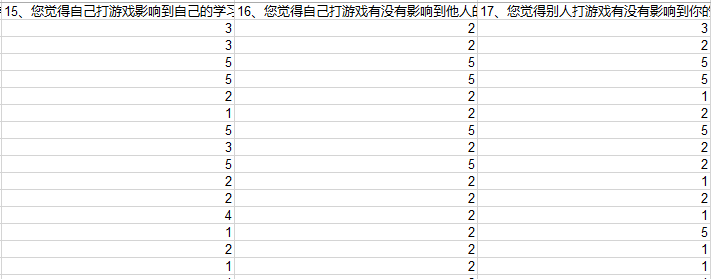
\includegraphics[width=.45\textwidth]{0}}
    $\quad$
    \subcaptionbox{Agter data pre-processing\label{F:Data-1-2}}%
        {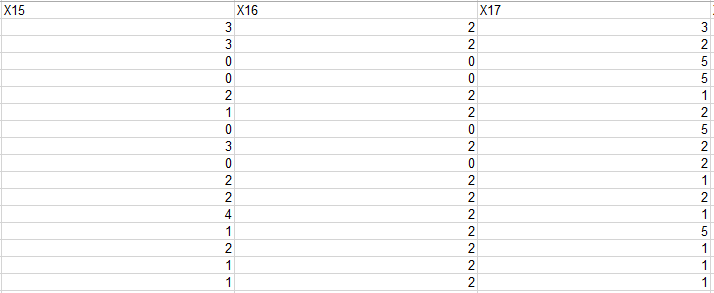
\includegraphics[width=.42\textwidth]{1}}
    \caption{Data with and without pre-processing}\label{F:Data-1}
\end{figure}

On the other hand, the options of some other questions (question 8 and 14) does not show apparent degree increasing. Therefore, we use dummy variables to represent different options. Figure~\ref{F:Data-2-1} and
figure~\ref{F:Data-2-2} have shown this pre-processing.

\begin{figure}[H]
    \centering
    \subcaptionbox{Before data pre-processing\label{F:Data-2-1}}%
        {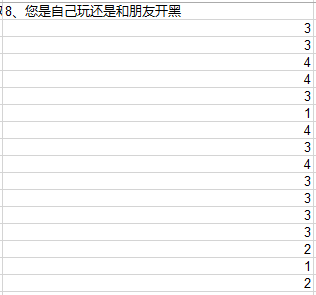
\includegraphics[width=.35\textwidth]{2}}
    $\quad$
    \subcaptionbox{After data pre-processing\label{F:Data-2-2}}%
        {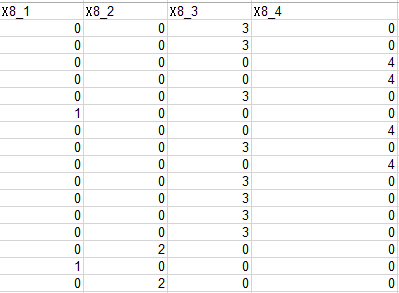
\includegraphics[width=.45\textwidth]{3}}
    \caption{Data with and without pre-processing}\label{F:Data-2}
\end{figure}



\section{Data Analysis}
\subsection{Correlation Matrix}
Before data prior processing, correlation matrix of all variables is plotted as figure~\ref{F:Data-3-1}. As the plot shown, this plot could not represent the correlation of different factors with playtime very well. Figure~\ref{F:Data-3-2} shows the correlation matrix after data prior processing. The correlation of various factors with playtime could be analysis evidently. Furthermore, we delete some factors that have few correlation
with playtime, which is exhibited as figure~\ref{F:Data-3-3}.

From figure~\ref{F:Data-3-2}, we can find more factors that correlated to playtime compared to figure~\ref{F:Data-3-1} ($X_5$
represents playtime). From figure~\ref{F:Data-3-1} we find play $\mathrm{MOBA}(X_6^{(1)})$ has the strongest correlation with
playtime, which means $\mathrm{MOBA}$ is the most addictive game type; while single-player game($X_6^{(5)}$) is the least addictive game type since it has the weakest correlation with playtime. Since $X_7^{(2)}$, $X_7^{(3)}$, $X_7^{(4)}$ have positive correlation with playtime,we can safely draw the conclusion that students who love game tend to spend more time on playing computer games.

\begin{analysis}{Negative correlation analysis}{negative-correlation}
From correlation matrix figure~\ref{F:Data-3-3}, we can find factors ``Nonplayer'', ``Nonplayer$_1$'', ``Nonplayer$_2$'', ``W hetherstay−uptoplay'', ``Condition$_5$'', ``Reasonforstayup$_2$'' have strong negative correlation with ``PlayTime''.
\end{analysis}

There is an interpretation of this conclusion. It is reasonable that non-player will have a shorter play time. Setting the value of stay-up to play games be 1 and not stay-up to play games be 3, we find out that the larger the value of this factor is, the smaller the value of playtime is, which is coincident with the fact that students who don't stay-up to play tend to have a shorter playtime. ``Condition$_5$'' and ``Reasonforstay-up$_2$'' also represent situations that students would not stay-up to play games.

\begin{analysis}{Positive correlation analysis}{positive-correlation}
``Play time'' is positively correlated with ``plan'' and ``settle time'', that is, those who have no plans and who often stay up late tend to spend more time on games. ``Play time'' positively correlated with $X_{13}$ and $X_{14}^{(1)}$ also prove this conjecture. Comparing ``Play time'' with $X_{15}$ and $X_{16}$, we conclude that those who care about their lives or others also have less game time.
\end{analysis}

\begin{figure}[H]
    \centering
    \subcaptionbox{Before data prior processing\label{F:Data-3-1}}%
        {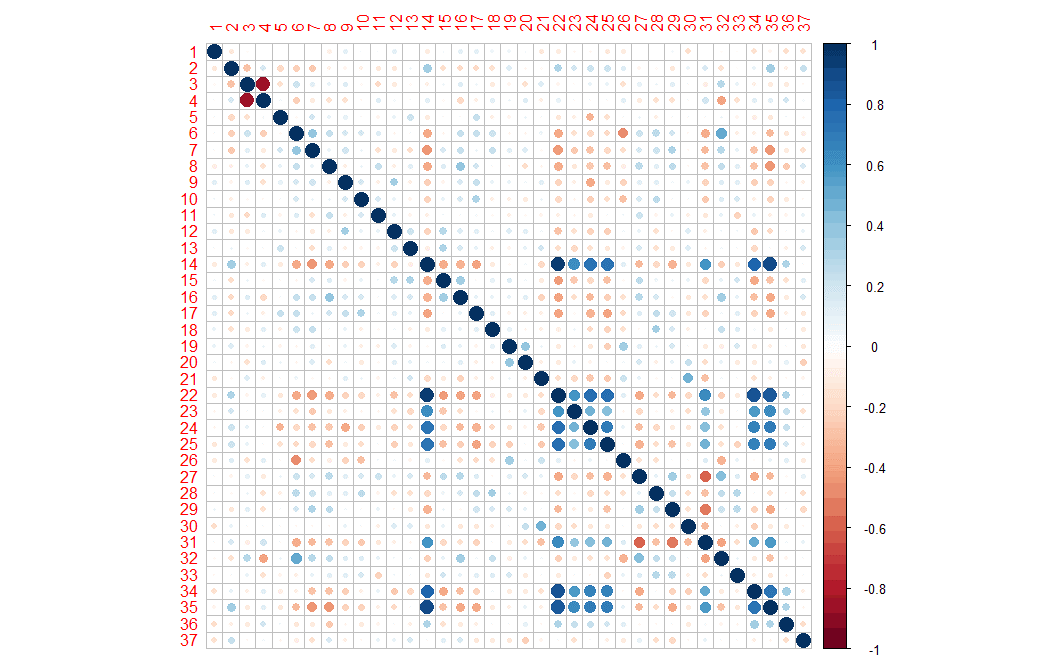
\includegraphics[width=.45\textwidth]{4}}
    $\quad$
    \subcaptionbox{After data prior processing\label{F:Data-3-2}}%
        {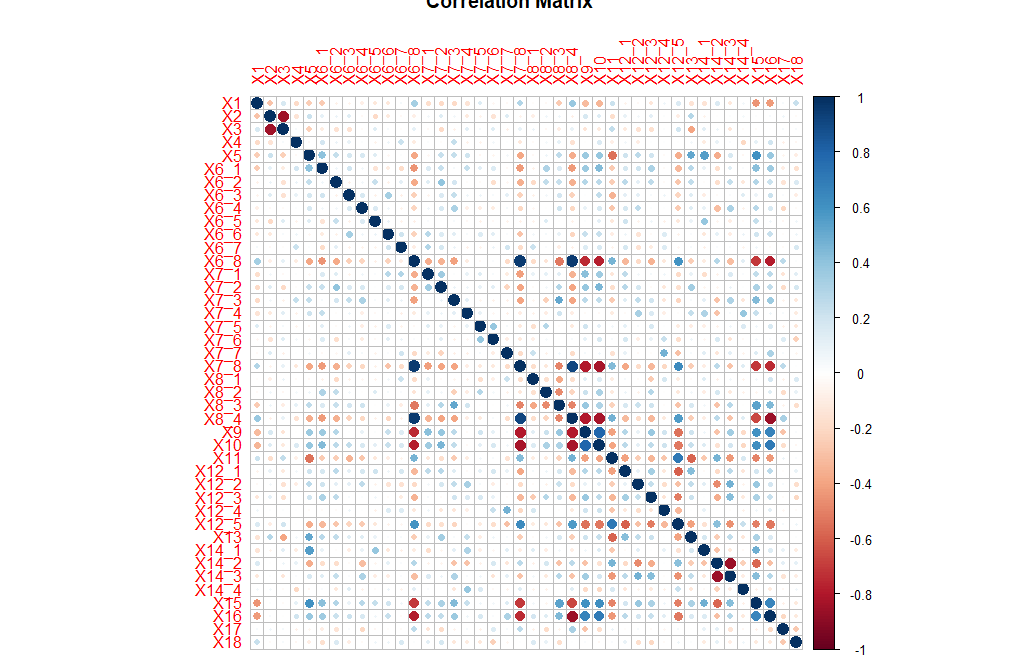
\includegraphics[width=.45\textwidth]{5}} \\
    \subcaptionbox{After deleting unsignificant data\label{F:Data-3-3}}%
        {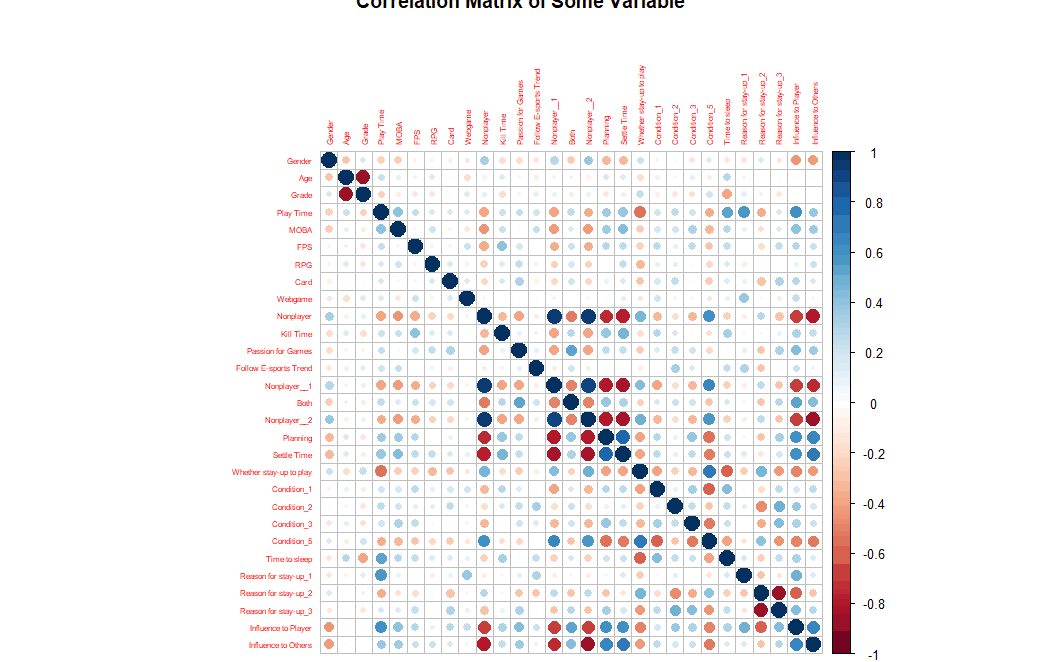
\includegraphics[width=.45\textwidth]{6}}
    \caption{Data with and without prior processing}\label{F:Data-3}
\end{figure}


\subsection{Wilcox Test of Playtime Between Different Grades}
We utilize wilcox test to judge whether there exist difference between distinguish grades' average playtime.

From wilcox test, we conclude that there are not sufficient evidences to reject the null hypothesis, that is, for grade$_1$ and grade$_2$, grade$_1$ and grade$_3$, grade$_2$ and grade$_3$, grade$_2$ and grade$_4$, there are no difference between these grade pairs' average playtime.

However, there are sufficient evidences to reject null hypothesis for grade$_3$ and grade$_4$ as long as grade$_1$ and grade$_4$, which means that there are clearly differences between these grade pairs' average playtime.


\subsection{Quantitative Analysis}
Average game time for four grades(senior, junior, sophomore, freshman) are respectively 20.21, 7.14, 12.72 and 7.55. Estimated playtime for students in \SUSTech\ is 11.07 hours per week. Boxplot of playtime vs. the grades are shown as figure~\ref{F:Data-4}.
\begin{equation}\label{E:temp-1}
    \bar{y}_{st} = \frac{1}{N}\sum_{i=1}^{L}N_i\bar{y}_i
\end{equation}

Applying the CLT, $\tfrac{\bar{y}-\mu}{\sqrt{\mathrm{Var}(\bar{y}_{st})}}\sim N(0,1)$. Thus a 95\%  confidence interval for the estimated game time is $[8.08,14.05]$. The 95\% confidence interval for the average game time for the four grades(senior, junior, sophomore, freshman) are respectively $[11.03,29.40]$, $[3.76,10.53]$, $[5.89,19.55]$ and $[2.60,12.48]$

\begin{figure}[H]
    \centering
    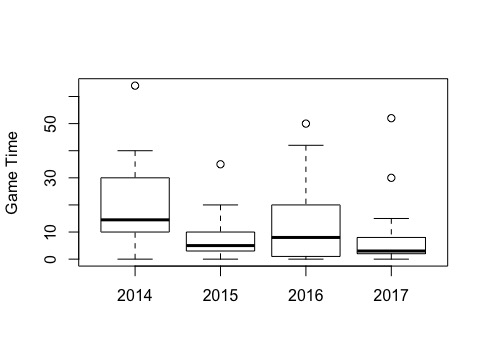
\includegraphics[width=.7\textwidth]{7}
    \caption{Boxplot of gametime vs. the grades}\label{F:Data-4}
\end{figure}

As it is shown in the correlation plot, playtime and MOBA player are positively correlated, box-plot of MOBA players' game time and non-MOBA players' game time are shown as figure~\ref{F:Data-5}:
\begin{figure}[H]
    \centering
    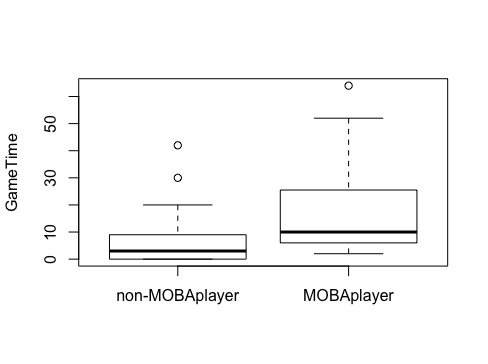
\includegraphics[width=.7\textwidth]{8}
    \caption{Gametime vs. MOBA}\label{F:Data-5}
\end{figure}

A Wilcoxon test is taken and the result is shown as figure~\ref{F:Data-6}. P-value is less than 0.01, it can be
concluded that MOBA players' game time is greater than non-MOBA players' playtime with confidence level 0.99. This result implies that MOBA players' playtime tends to be longer.
\begin{figure}[H]
    \centering
    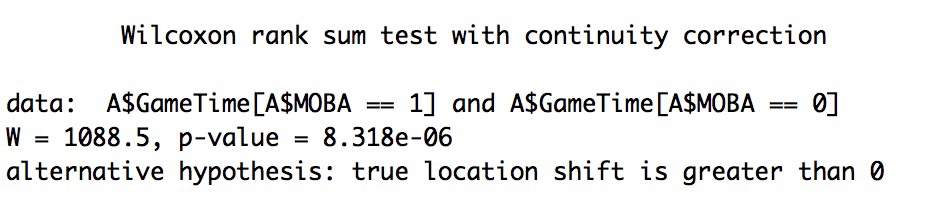
\includegraphics[width=.7\textwidth]{9}
    \caption{Correlation between parameters}\label{F:Data-6}
\end{figure}

Another pair of highly negatively correlated parameters are game time and gender, it suggests the understandable conclusion that boys' game time is much longer than girls' game time.



\section{Superiority and Weakness}
\begin{analysis}{Superiority}{superiority}
From above analysis, we know that the sample mean for playtime spent on games is an unbiased estimator. Furthermore, we obtain a prior sample variance of each grade to identify the sample size $n$.
\end{analysis}

\begin{analysis}{Weakness}{weakness}
There are also some problems that will effect the accuracy of result. Firstly, there exists missing data in sample, we didn't find a proper way to process these data. Secondly, we think that
the sampling method will lose a little precision for the reason that some questions are too subjective.
\end{analysis}



\section{Summary}
Our analysis on data can mainly divided into three parts.

\begin{analysis}{Prior Analysis}{prior-analysis}
Firstly, we performed the prior analysis on data, in this section we determined the sample size $n_i$ for each grades such that the estimated average playtime is within an error bound $B$.
\end{analysis}

\begin{analysis}{Qualitative Analysis}{qualitative-analysis}
Secondly, we performed the qualitative analysis on data, in this section we first reset the value of some variables to make it meaningful for the aim to get the correlation matrix. From the pictures above we can clearly point out that whether playing MOBA games is the biggest factor affecting the playtime. Furthermore, we can also conclude that boy's playtime is much longer than girl's playtime.
\end{analysis}

\begin{analysis}{Quantitative Analysis}{quantitative-analysis}
Last, we perform the quantitative analysis. In this section, we mainly analysis the value of playtime for each grades. We first calculate the mean value and the confidence interval, then we perform a wilcoxon rank test for all four mean values of playtime for four grades, from which we can conclude that there are clearly difference between the average playtime  for the two pairs: grade$_3$ and grade$_4$, grade$_1$ and grade$_4$.
\end{analysis}

\end{document}
